\documentclass{article}
\usepackage[utf8]{inputenc}
\usepackage{amsmath}
\usepackage{ifsym}
\usepackage{pythonhighlight}
\usepackage{graphicx}
\usepackage[a4paper, total={6in, 8in}]{geometry}

\usepackage{listings}
\usepackage{color}

\definecolor{dkgreen}{rgb}{0,0.6,0}
\definecolor{gray}{rgb}{0.5,0.5,0.5}
\definecolor{mauve}{rgb}{0.58,0,0.82}

\lstset{frame=tb,
  language=Java,
  aboveskip=3mm,
  belowskip=3mm,
  showstringspaces=false,
  columns=flexible,
  basicstyle={\small\ttfamily},
  numbers=none,
  numberstyle=\tiny\color{gray},
  keywordstyle=\color{blue},
  commentstyle=\color{dkgreen},
  stringstyle=\color{mauve},
  breaklines=true,
  breakatwhitespace=true,
  tabsize=3}
  
\title{Labwork 3 - Image grayscale transformation using Numba Cuda}
\author{Nguyen Le Tuan Duy - M21.ICT.004}
\date{}



\begin{document}

\maketitle
\section{Load and Flatten the Image}
The first step is to load the image, calculate the total of pixel and then flatten it using the reshape function and the number of pixel that has just calculated:

\begin{python}
img = Image.open('000054.JPG')
img.save('sample.png')
 
numpy_img = np.asarray(img)

PixCount = numpy_img.shape[0]* numpy_img.shape[1]


numpy_img = numpy_img.reshape(PixCount,3)
\end{python}

\begin{figure}
    \begin{center}
        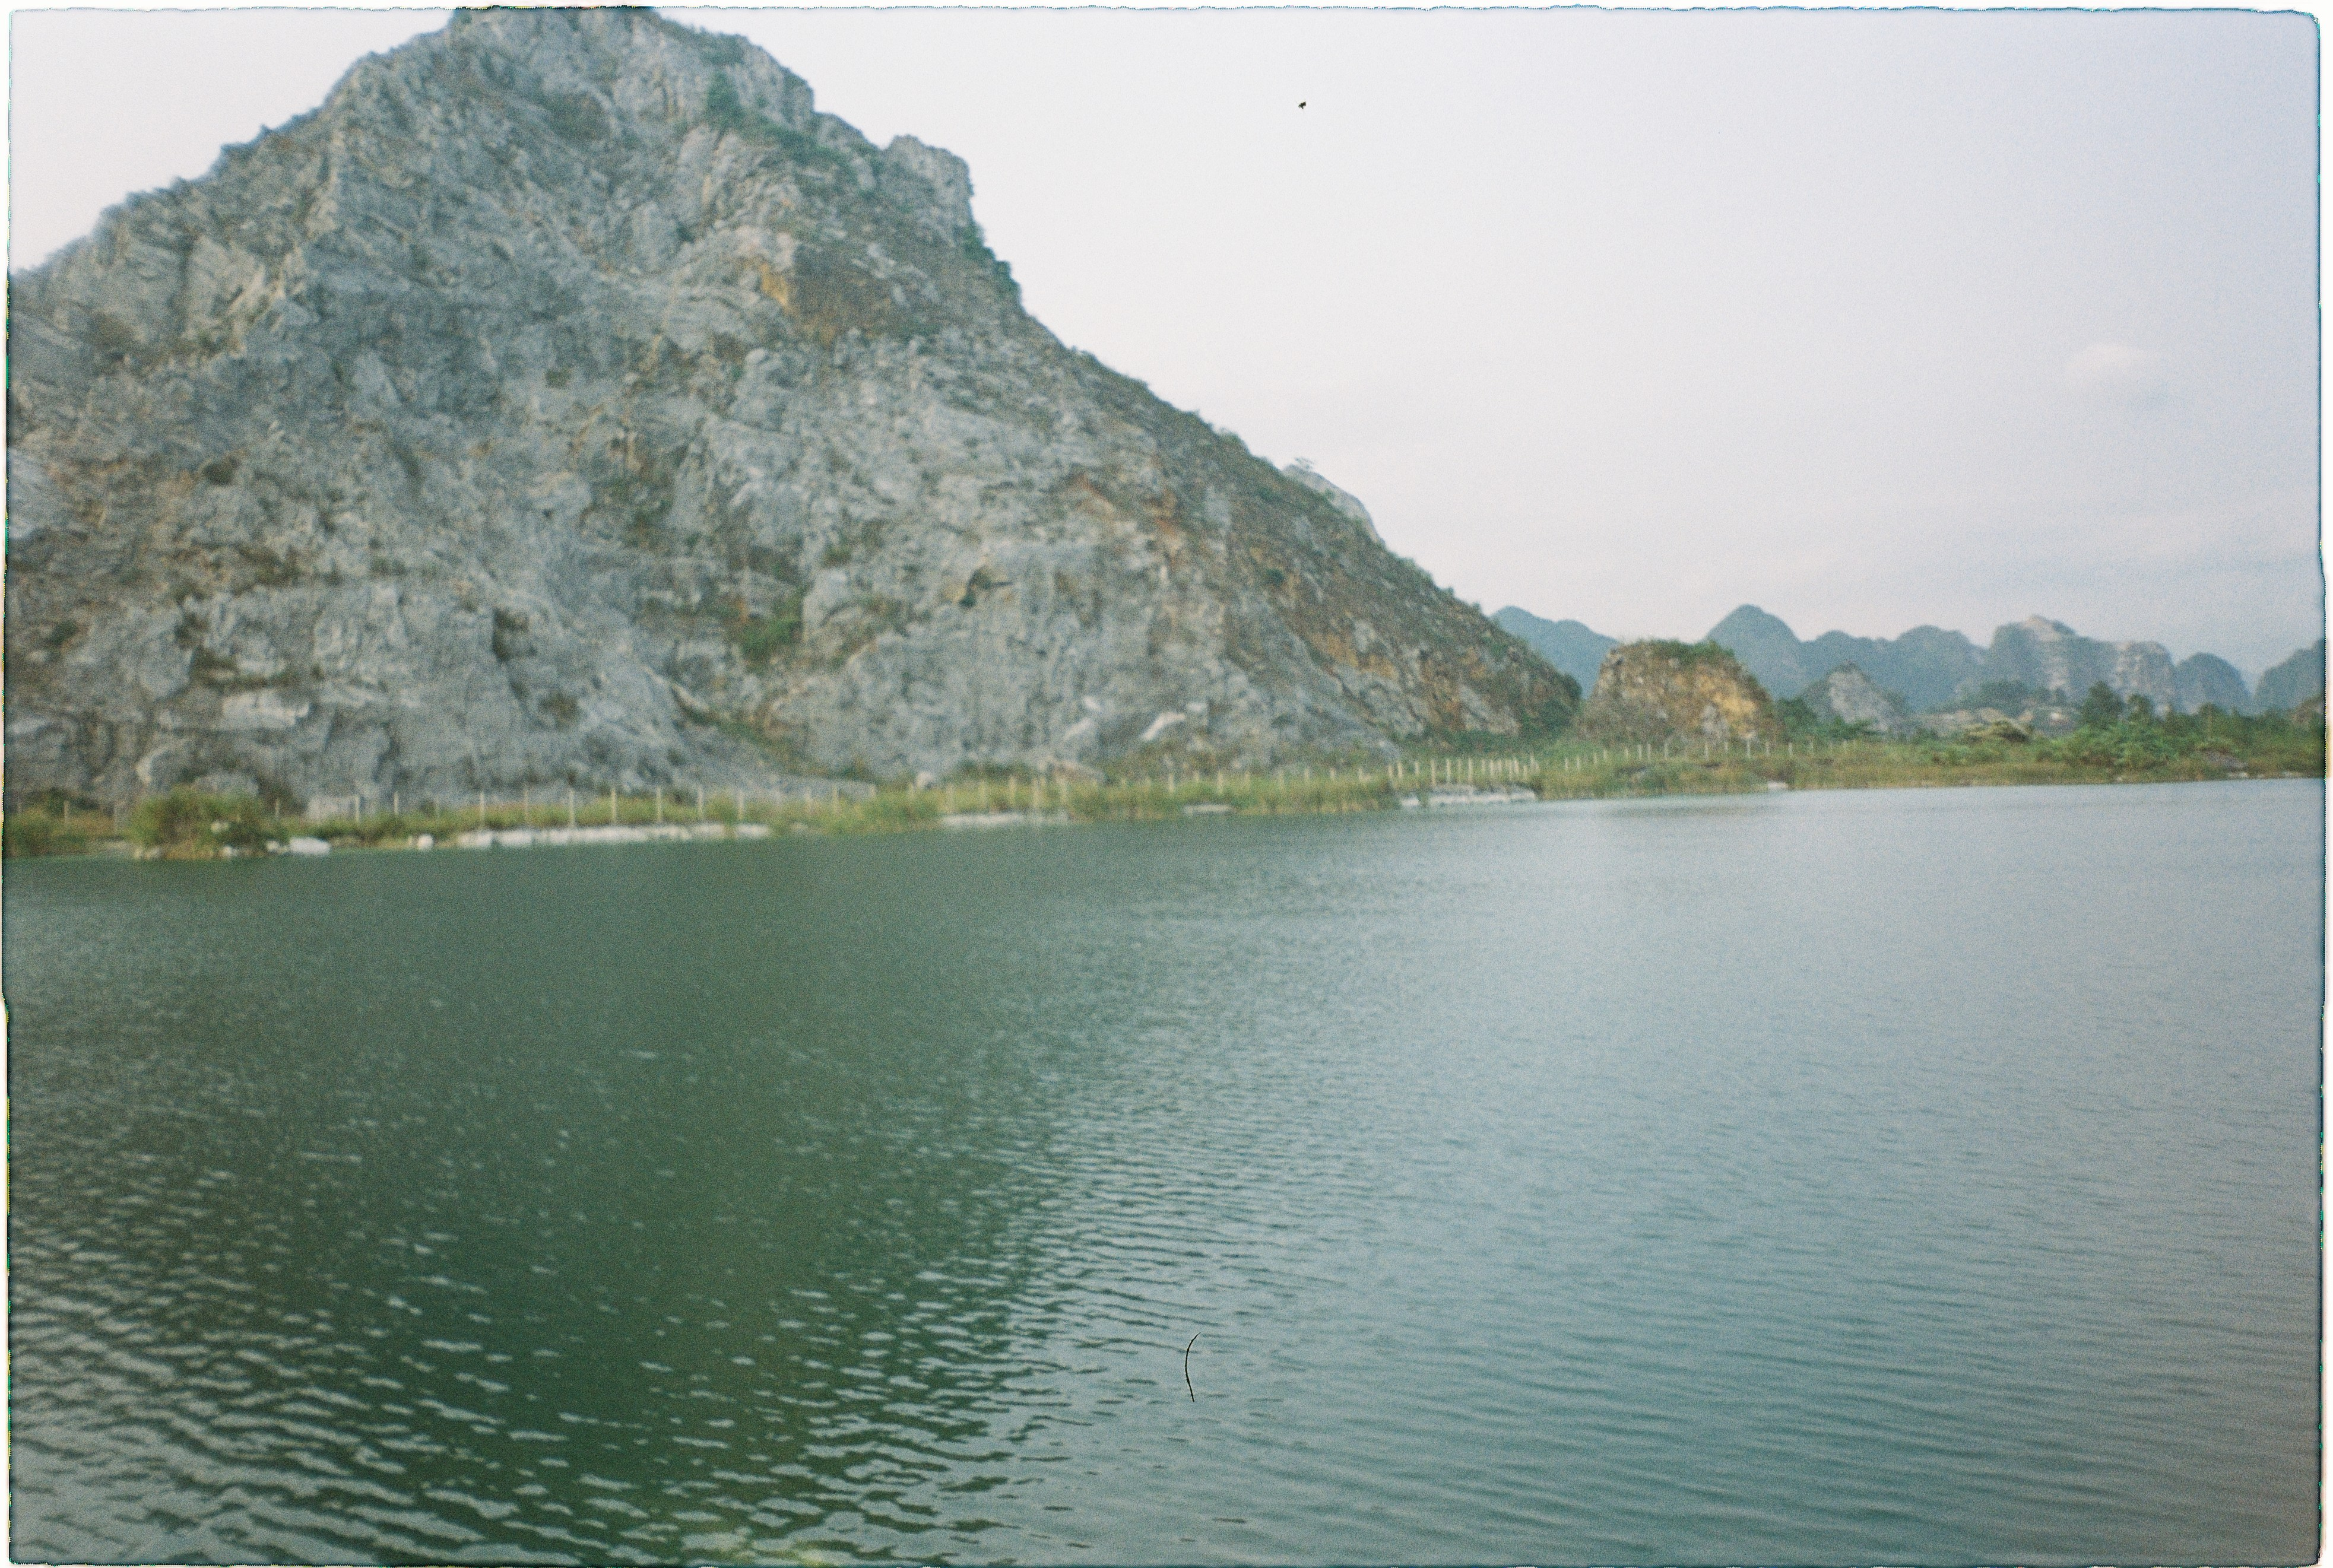
\includegraphics[scale=0.08]{000054.JPG}
        \caption{Original image}
    \end{center}
\end{figure}

The formula that we will use for grayscaling image averaging the 3 value of R, G, B of each pixel:
\begin{equation}
    g(y,x) = \frac{1}{3}\sum_{i=0}^{3}I(y,x,i)
\end{equation}

\section{Grayscalling image using CPU}
Function for CPU is just some simple manipulation on Numpy array:
\begin{python}
def cpu_greyscale(img):
  new_img = np.zeros((img.shape[0]))
  for i in range(len(img)):
    pixel = 0
    for j in range(3):
      pixel += img[i][j]
    pixel = pixel /3
    new_img[i] = pixel
  return(new_img)
\end{python}

Then we calculate the time, reshape again into 2D image and display it:
\begin{python}
time1 = time.time()
greyscale_img = cpu_greyscale(numpy_img)
print('CPU time in seconds: ', time.time()-time1)


greyscale_img = greyscale_img.reshape(2642,3930)
output_img = Image.fromarray(greyscale_img)
plt.imshow(greyscale_img, cmap='gray', vmin=0, vmax=255)
plt.show()
\end{python}

\section{Grayscalling image using GPU}
Define the function:
\begin{python}
@cuda.jit
def GPU_grayscale(src, dst):
    tidx = cuda.threadIdx.x + cuda.blockIdx.x * cuda.blockDim.x
    g = (src[tidx, 0] + src[tidx, 1] + src[tidx, 2])/3
    dst[tidx] = g
\end{python}

Initialization by loading and allocating memory into the GPU:
\begin{python}
blocksize = 64
blocksize_range = [16,32,64,128,256,512,1024]
devOutput = cuda.device_array((PixCount), np.float64)
devInput = cuda.to_device(numpy_img)
\end{python}

Trying to check with different block size:

\begin{python}
for blocksize in blocksize_range:
  gridSize = math.ceil(PixCount / blocksize)
  time1 = time.time()
  GPU_grayscale[gridSize, blocksize](devInput, devOutput)
  print('GPU time in seconds of blocksize ',blocksize,' : ', time.time()-time1)
\end{python}

Finally copy the output back and display the image:
\begin{python}
hostOutput = devOutput.copy_to_host()

greyscale_img = hostOutput.reshape(2642,3930)
plt.imshow(greyscale_img, cmap='gray', vmin=0, vmax=255)
plt.show()
\end{python}

\section{Result}
The output image is successfully greyscale image when using with both CPU and GPU
\begin{figure}
    \begin{center}
        \includegraphics[scale=1]{output_grey.png}
        \caption{Output greyscale image}
    \end{center}
\end{figure}

\newpage
\begin{table}
\caption{Times in different settings}
\begin{tabular}{|c|c|c|c|c|c|c|c|c|}
\hline
\bfseries Type of running &CPU  &GPU16  &GPU32   &GPU64   &GPU128    &GPU256   &GPU512   &GPU1024     \\
\hline\hline
\bfseries Time in seconds     &35.41   &0.23 &0.021 &0.018 &0.02 &0.019 &0.024 &0.019    \\
\hline
\end{tabular}
\end{table} 
We can see that the first time we use GPU, the time is slowly but from that the speed is much better due to the cache already ultilizies. In all case, the speed still extremely faster than CPU. Different block size dont illustrate much changes in this case.
\end{document}